\section{数制}

\begin{frame}\ft{\secname}
\begin{defn}{}
数制也称计数制,是用一组固定的符号和统一的规则来表示数值的方法。通常采用的数制有十进制、二进制、八进制和十六进制。
\end{defn}
\vspace{0.2in}

在一种数制中,只能使用一组固定的数字符号来表示数目的大小。具体使用多少个数字符号来表示数目的大小,就称为该数制的基数。
\end{frame}

\begin{frame}\ft{\secname}
\begin{itemize}
\item 十进制(Decimal)
\item[]
  基数是10,有10个数字符号,即0,l,2,3,4,5,6,7,8,9。\\[0.1in]
\item 二进制(Binary)
\item[]
  基数是2,只有两个数字符号,即0和1。\\[0.1in]
\item 八进制(Octal)
\item[]
  基数是8,它有8个数字符号,即0,l,2,3,4,5,6,7。\\[0.1in]
\item 十六进制(Hexadecimal)
\item[]
  基数是16,它有16个数字符号,除了十进制中的10个数外,还使用了6个英文字母。16个数字符号依次是
  $$\mbox{0,~1,~2,~3,~4,~5,~6,~7,~8,~9,~A,~B,~C,~D,~E,~F.}$$
  其中A$\sim$F分别代表十进制数的10$\sim$15。
\end{itemize}
\end{frame}




\begin{frame}\ft{\secname}
\begin{figure}[h]
\centering
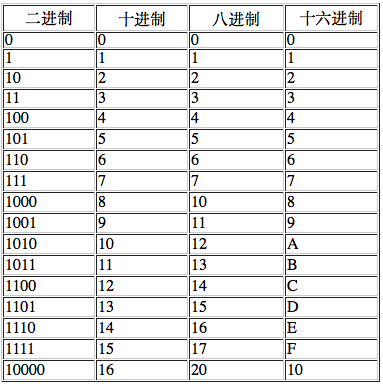
\includegraphics[width=3.in]{slide01/images/shuzhi}
\end{figure}
\end{frame}

\begin{frame}\ft{进制}
\red{在数制中,N进制必须是逢N进一。}

\begin{itemize}
\item 十进制数
\[
(1010)_{10}=1\times10^3+0\times10^2+1\times10^1+0\times10^0
\]
\item 二进制数
\[
(1010)_{2}=1\times2^3+0\times2^2+1\times2^1+0\times2^0=(10)_{10}
\]
\item 八进制数
\[
(1010)_{8}=1\times8^3+0\times8^2+1\times8^1+0\times8^0=(520)_{10}
\]
\item 十六进制数
\[
\mbox{(BAD)}_{16}=11\times16^2+10\times16^1+13\times16^0=(2989)_{10}
\]
\end{itemize}
\end{frame}

\begin{frame}\ft{二进制数}

  \begin{free}[加法法则]{}
    \[
        \begin{array}{l}
          0+0=0\\
          0+1=1\\
          1+0=1\\
          1+1=10\\
          1+1+1=10+1=11
        \end{array}
    \]
  \end{free}

  \begin{exam}{}
    \begin{table}
      \centering
      \begin{tabular}{cD{.}{.}{3}}
        &1~0~1~1\\
        +&1~0~1~0\\
        \hline
        =&1~0~1~0~1
      \end{tabular}
    \end{table}
  \end{exam}
\end{frame}

\begin{frame}\ft{二进制数}
  \begin{free}[减法法则]{}
    \[
      \begin{array}{rl}
        0-0=0&\\
        1-0=1&\\
        1-1=0&\\
        0-1=1&\mbox{有借位,借1当$(10)_2$}\\
        0-1-1=0&\mbox{有借位}\\
        1-1-1=1&\mbox{有借位}\\
      \end{array}
    \]
  \end{free}

  \begin{exam}{}
    \begin{table}
      \centering
      \begin{tabular}{cD{.}{.}{3}}
        % &111110\\
          &1~1~0~0~0~0\\
        -&1~0~1~1~1\\
        \hline
        =&1~1~0~0~1
      \end{tabular}
    \end{table}
  \end{exam}
\end{frame}

\begin{frame}\ft{二进制数}

  \begin{free}[乘法法则]{}
    \[
      \begin{array}{rr}
        0\times0=0, & 
                      0\times1=0\\
        1\times0=0, & 
                      1\times1=1\\
      \end{array}
    \]
  \end{free}

  \begin{exam}{}
    \begin{table}
      \centering
      \begin{tabular}{cD{.}{.}{3}}
        % &111110\\
          &1~1~1~0\\
        $\times$&0~1~1~0\\
        \hline
          &0~0~0~0\\
          &1~1~1~0~~~\\
          &1~1~1~0~~~~~\\
        +&0~0~0~0~~~~~~~~\\
        \hline
          &1~0~1~0~1~0~0
      \end{tabular}
    \end{table}
  \end{exam}

\end{frame}
%
\begin{frame}\ft{二进制数}

  \begin{figure}
    \centering
    \begin{tikzpicture}
      \matrix[ampersand replacement=\&,matrix of math nodes,nodes={inner sep=0.2em}]{
        \& \& \& \&  \& 1 \& 1 \& 0 \& 1\\[4pt]
        110 \& \sqrt{} \& |(a)|1\& 0 \& 0\& 1 \& 1 \& 1 \& |(b)| 0 \\
        \& - \&  |(c)| \&  1 \& 1\& |(d)|0  \&  \&  \&   \\[4pt]
        \&   \&   \&   \& 1\& 1  \& 1\&  \&   \\[4pt]
        \& - \&   \&   \& |(e)|1\& 1  \& |(f)|0\&  \&   \\[4pt]
        \&   \&   \&   \&  \&    \& 1\& 1\& 0  \\[4pt]
        \& - \&   \&   \&  \&    \& |(g)|1\& 1\& |(h)|0  \\[4pt]
        \&   \&   \&   \&  \&    \&  \&  \& 0  \\[4pt]
      };
      \draw[thick] (a.north west) -- (b.north east)
      (c.south west) -- (d.south east)
      (e.south west) -- (f.south east)
      (g.south west) -- (h.south east);

    \end{tikzpicture}
    \caption{二进制数的除法}
  \end{figure}
\end{frame}

\begin{frame}\ft{十进制转二进制}

  \begin{free}[整数部分]{}
    除2取余,直至商为0,最后将所得余数按逆序排列。 
  \end{free}

  \begin{exam}{}
    \begin{figure}
      \centering
      \begin{tikzpicture}
        \matrix[ampersand replacement=\&,matrix of math nodes,column sep=1ex,nodes={inner sep=0.2em}]{
          2  \& |(a)|  2 \& |(b)|3 \& \& \& \\[4pt]
          2  \& |(c)|  1 \& |(d)|1 \& \& \& \blue{1}\\[4pt]
          \&        2 \& |(e)|5 \& \& \& \blue{1}\\[4pt]
          \&        2 \& |(f)|2 \& \& \& \blue{1}\\[4pt]
          \&        2 \& |(g)|1 \& \& \& \blue{0}\\[4pt]
          \&          \&      0 \& \& \& \blue{1}\\[4pt]
        };
        \draw[thick] (a.north west)--(a.south west)--(b.south east)
        (c.north west)--(c.south west)--(d.south east)
        (e.north west)--(e.south west)--(e.south east)
        (f.north west)--(f.south west)--(f.south east)
        (g.north west)--(g.south west)--(g.south east);
      \end{tikzpicture}
      \caption{ $(23)_{10}=(10111)_2$}
    \end{figure}
  \end{exam}
\end{frame}
%
\begin{frame}\ft{十进制转二进制}

  \begin{free}[小数部分]{}
    乘2取整数,若小数部分是5的倍数,则以最后小数部分为0为止,否则以约定的精确度为准,最后将所取整数按顺序排列。 
  \end{free}
  
  \begin{exam}{}
    \begin{figure}
      \centering
      \begin{tikzpicture}
        \matrix[ampersand replacement=\&,matrix of math nodes,column sep=1ex,nodes={inner sep=0.2em}]{
          \& 0 \& .\& 2\& 5      \& \&  \\[4pt]
          |(a)|\times \&   \&  \&  \& |(b)|2 \& \&   \\[4pt]
          \& 0 \& .\& 5\& 0      \& \& \mbox{取整数位}0 \\[4pt]
          |(c)|\times \&   \&  \&  \& |(d)|2 \& \&   \\[4pt]
          \& 1 \& .\& 0\& 0      \& \& \mbox{取整数位}1  \\[4pt]        
        };
        \draw[thick] (a.south west)--(b.south east)
        (c.south west)--(d.south east);
      \end{tikzpicture}
      \caption{$(0.25)_{10}=(0.01)_2$}
    \end{figure}
  \end{exam}
\end{frame}
%
\begin{frame}\ft{十进制转二进制}
  \begin{exam}{}
    将十进制数$125.24$转换为二进制数(取四位小数)。
  \end{exam}
  \pause 

  \begin{figure}
    \begin{minipage}[t]{0.45\linewidth}
      \centering
      \begin{tikzpicture}[scale=0.8]
        \matrix[ampersand replacement=\&,matrix of math nodes,column sep=1ex,nodes={inner sep=0.2em}]{
          2  \& |(a)|  1 \&       2 \& |(b)|5 \& \& \& \\[4pt]
          2  \& |(c)|  1 \&       6 \& |(d)|2 \& \& \& \blue{1}\\[4pt]
          \&        2 \& |(e1)|3 \& |(e)|1 \& \& \& \blue{0}\\[4pt]
          \&        2 \& |(f1)|1 \& |(f)|5 \& \& \& \blue{1}\\[4pt]
          \&          \&       2 \& |(g)|7 \& \& \& \blue{1}\\[4pt]
          \&          \&       2 \& |(h)|3 \& \& \& \blue{1}\\[4pt]
          \&          \&       2 \& |(i)|1 \& \& \& \blue{1}\\[4pt]       
          \&          \&         \&      0 \& \& \& \blue{1}\\[4pt]
        };
        \draw[thick] (a.north west)--(a.south west)--(b.south east)
        (c.north west)--(c.south west)--(d.south east)
        (e1.north west)--(e1.south west)--(e.south east)
        (f1.north west)--(f1.south west)--(f.south east)
        (g.north west)--(g.south west)--(g.south east)
        (h.north west)--(h.south west)--(h.south east)
        (i.north west)--(i.south west)--(i.south east);

      \end{tikzpicture}
    \end{minipage}
    \hfill
    \begin{minipage}[t]{0.45\linewidth}
      \centering
      \begin{tikzpicture}[scale=0.8]
        \matrix[ampersand replacement=\&,matrix of math nodes,column sep=1ex,nodes={inner sep=0.1em}]
        {
          \& 0 \& .\& 2\& 4      \& \&  \\[4pt]
          |(a)|\times \&   \&  \&  \& |(b)|2 \& \&   \\[4pt]
          \& 0 \& .\& 4\& 8      \& \& \mbox{取整数位}0 \\[4pt]
          |(c)|\times \&   \&  \&  \& |(d)|2 \& \&   \\[4pt]
          \& 0 \& .\& 9\& 6      \& \& \mbox{取整数位}0  \\[4pt]
          |(e)|\times \&   \&  \&  \& |(f)|2 \& \&   \\[4pt]
          \& 1 \& .\& 9\& 2      \& \& \mbox{取整数位}1  \\[4pt]                    
          |(g)|\times \&   \&  \&  \& |(h)|2 \& \&   \\[4pt]
          \& 1 \& .\& 8\& 4      \& \& \mbox{取整数位}1  \\[4pt]            
        };
        \draw[thick] (a.south west)--(b.south east)
        (c.south west)--(d.south east)
        (e.south west)--(f.south east)
        (g.south west)--(h.south east);
      \end{tikzpicture}
    \end{minipage}
  \end{figure}
  \pause 
  结果为
  $$
  (125.24)_{10}=(1111101.0011)_2.
  $$
\end{frame}
%
% \begin{frame}\ft{二进制转十进制}

% \begin{free}[基本原理]{}
%   \begin{itemize}
%   \item 将二进制数从小数点开始,往左从$0$开始对各位进行正序编号,往右序号则分别为$-1,-2,-3,\cd$,直到最末位。\\[0.1in]
%   \item 然后分别将各位上的数乘以$2$的$k$次幂所得的值进行求和,其中$k$的值为各个位所对应的上述编号。
%   \end{itemize}
% \end{free} 
% \end{frame}

\begin{frame}\ft{二进制转十进制}
  \begin{exam}{}
    将$(1101.101)_2$转换为十进制数。
  \end{exam}
  \pause 
  $$
  \begin{array}{rl}
    & (1101.101)_2 \\[0.1in]
    = & 1\times2^3+1\times2^2+0\times2^1+1\times2^0
        +1\times2^{-1}+0\times2^{-2}+1\times2^{-3}\\[0.1in]
    = & 8+4+1+0.5+0.125\\[0.1in]
    = & 13.625
  \end{array}
  $$
\end{frame}
%
% \begin{frame}\ft{二进制转十六进制}

% \red{基本原理:} 由于十六进制数基数是2的四次幂,所以一个二进制转换为十六进制,
% \begin{itemize}
% \item
% 如果是整数,只要从它的低位到高位每$4$位组成一组,然后将每组二进制数所对应的数用十六进制表示出来。\\[0.1in]
% \item
% 如果有小数部分,则从小数点开始,分别向左右两边按照上述方法进行分组计算。
% \end{itemize}
% \end{frame}
%
\begin{frame}\ft{二进制转十六进制}
  \begin{exam}{}
    将$(11~1010~1111~0001~0111)_2$转换为十六进制数。
  \end{exam}
  \pause 
  \begin{table}
    \centering
    \begin{tabular}{cccccc}\hline
      二进制数&$11$&$1010$&$1111$&$0001$&$0111$\\[0.1in]
      十六进制数&$3$&$A$&$F$&$1$&$7$\\ \hline
    \end{tabular}
  \end{table}
  结果为
  $$
  (11~1010~1111~0001~0111)_2=(3AF17)_{16}
  $$
\end{frame}
%
%
